\documentclass{lmcs} %%% last changed 2014-08-20

%% mandatory lists of keywords
\keywords{BPMN, Higher-order model transformation, Graph transformation, Model checking, Formalization}
% My packages
\usepackage{amssymb} % \square command
% Footnotes inside tables
\usepackage{footnote}
\usepackage{csquotes} % enquote command
\usepackage{glossaries} % Glossary
\usepackage{threeparttable} % Tables with notes
\makesavenoteenv{tabular}
\makesavenoteenv{table}
% Acronyms
\newacronym{bpmn}{BPMN}{Business Process Modeling Notation}
\newacronym{gt}{GT}{Graph Transformation}
\newacronym{mt}{MT}{Model Transformation}
\newacronym{hot}{HOT}{Higher-Order model Transformation}
% My packages end

\usepackage{hyperref}

\def\eg{{\em e.g.}}
\def\cf{{\em cf.}}
\def\ie{{\em i.e.}}

\begin{document}

\title[Formalization and analysis of BPMN using graph transformation systems]{A higher-order approach to the formalization and analysis of BPMN using graph transformation systems\rsuper*}
\titlecomment{{\lsuper*}This article is an extended version of \cite{krauterFormalizationAnalysisBPMN2023}}
% \thanks{thanks, optional.}	%optional

\author[T.~Kr\"{a}uter]{Tim Kr\"{a}uter\lmcsorcid{0000-0003-1795-0611}}[a]
\author[A.~Rutle]{Adrian Rutle\lmcsorcid{0000-0002-4158-1644}}[a]
\author[H.~K\"{o}nig]{Harald K\"{o}nig\lmcsorcid{0000-0001-6304-6311}}[a,b]
\author[Y.~Lamo]{Yngve Lamo\lmcsorcid{0000-0001-9196-1779}}[a]

\address{Western Norway University of Applied Sciences, Bergen, Norway}
\email{tkra@hvl.no, aru@hvl.no, hkoe@hvl.no, yla@hvl.no}

\address{University of Applied Sciences, FHDW, Hanover, Germany}
\email{harald.koenig@fhdw.de}

%% etc.

%% required for running head on odd and even pages, use suitable
%% abbreviations in case of long titles and many authors:

%%%%%%%%%%%%%%%%%%%%%%%%%%%%%%%%%%%%%%%%%%%%%%%%%%%%%%%%%%%%%%%%%%%%%%%%%%%

%% the abstract has to PRECEDE the command \maketitle:
%% be sure not to issue the \maketitle command twice!

\begin{abstract}
  \noindent
The Business Process Modeling Notation (BPMN) is a widely used standard notation for defining intra- and inter-organizational workflows.
However, the informal description of the BPMN execution semantics leads to different interpretations of BPMN elements and difficulties in checking behavioral properties.
In this article, we propose a formalization of the execution semantics of BPMN that, compared to existing approaches, covers more BPMN elements while facilitating property checking.
Our approach is based on a higher-order transformation from BPMN models to graph transformation systems.
As proof of concept, we have implemented our approach in an open-source web-based tool.
\end{abstract}

% TODO: Archive repo with DOI using zenodo: https://docs.github.com/en/repositories/archiving-a-github-repository/referencing-and-citing-content

\maketitle
\section{Introduction}
In today's fast-paced business environment, organizations with complex workflows require a powerful means to accurately map, analyze, and optimize their processes. 
\gls*{bpmn} \cite{objectmanagementgroupBusinessProcessModel2013} is a widely used standard to define these workflows.
However, the informal description of the \gls*{bpmn} execution semantics leads to different interpretations of \gls*{bpmn} models and difficulties in checking behavioral properties \cite{corradiniFormalApproachAnalysis2021}.
Various studies have shown that business process models indeed suffer from control-flow errors \cite{mendlingEmpiricalStudiesProcess2009}.
Formalizing \gls*{bpmn} would reduce the cost of business process automation drastically by facilitating the detection of errors and optimization potentials in process models already during design time.
To this end, we propose a formalization that covers most of the \gls*{bpmn} elements used in practice and supports checking behavioral properties.
General behavioral properties such as \textit{Safeness} and \textit{Soundness} were adapted to \gls*{bpmn} \cite{corradiniClassificationBPMNCollaborations2018}, which can uncover potential flaws in \gls*{bpmn} models leading to deadlocks or other undesirable execution states.

In this article, we consider two fundamental concepts when formalizing the execution semantics of \gls*{bpmn}.
First, \textit{state structure}, \ie, how models are represented during execution.
The state structure corresponds to the type graph in \gls*{gt} systems.
Second, \textit{state-changing elements}, \ie, which elements in a model encode state changes.
These elements are implemented using \gls*{gt} rules.
In our approach, we automatically generate \gls*{gt} rules based on a \gls*{hot} for each specific \gls*{bpmn} model, as shown in \autoref{fig:approach}.

\begin{figure}[ht]
    \centering
    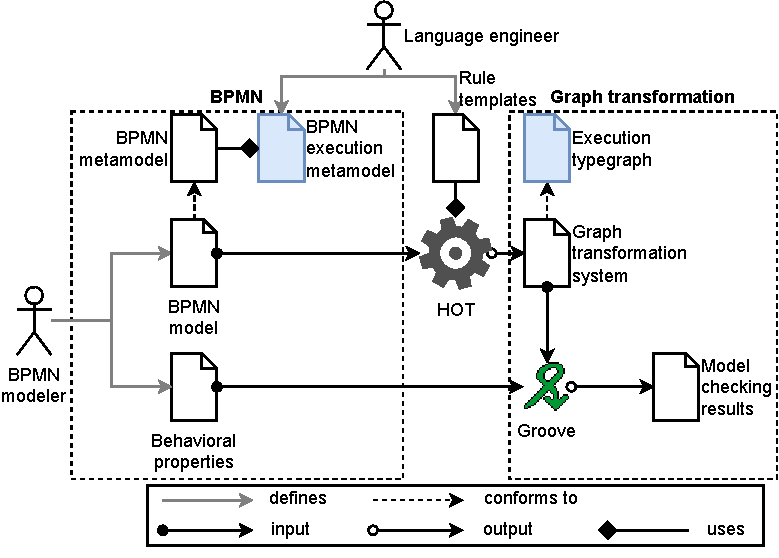
\includegraphics[width=0.8\textwidth]{images/bpmn_semantics-overview.pdf}
    \caption{Overview of the approach}
    \label{fig:approach}
\end{figure}

To begin the \gls*{bpmn} modeling process, a modeler first defines the \gls*{bpmn} model and its corresponding behavioral properties for evaluation.
This model must adhere to the \gls*{bpmn} metamodel as outlined in the \gls*{bpmn} specification by the Object Management Group \cite{objectmanagementgroupBusinessProcessModel2013}.
To create the state structure for BPMN, the \gls*{bpmn} execution metamodel is defined by language engineers, utilizing the \gls*{bpmn} metamodel as a foundation.
Typically, an execution metamodel is created by extending the languages metamodel.

Furthermore, we define a \gls*{hot} from \gls*{bpmn} models to \gls*{gt} systems.
We call the transformation \textit{higher-order} since the resulting graph-transformation systems represent model-transformations themselves \cite{tisiUseHigherOrderModel2009}.
The \gls*{hot} creates a \gls*{gt} system, \ie, \gls*{gt} rules and a start graph for a given \gls*{bpmn} model.
It is defined using rule generation templates, which describe how \gls*{gt} rules should be generated for each state-changing element in \gls*{bpmn} (see \autoref{sec:formalization}).
The obtained \gls*{gt} system conforms to the execution type graph, which corresponds to the \gls*{bpmn} execution metamodel.
In the figure, we have colored both artifacts blue to visualize that they contain the same information.
Ultimately, we use Groove as an execution engine for the \gls*{gt} system and check the behavioral properties defined earlier.

Our approach has been implemented in a user-friendly, open-source web-based tool, the \textit{\gls*{bpmn} Analyzer}, which can be used online without needing installation.
The \gls*{bpmn} Analyzer was validated using a comprehensive test suite.
Additionally, our approach is versatile as it can be applied to formalize other behavioral languages, such as activity diagrams, state charts, and more.
To define the execution semantics of an alternate behavioral language, one simply needs to establish a new execution metamodel and \gls*{hot} (see the language engineer in \autoref{fig:approach}).

% Contributions summary
The contribution of this article is twofold.
First, we introduce a new approach utilizing a \gls*{hot} to generate \gls*{gt} rules instead of providing fixed \gls*{gt} rules to formalize the semantics of a behavioral language.
Second, we apply our approach to \gls*{bpmn}, resulting in a formalization covering most \gls*{bpmn} elements that supports property checking.

% Compared to the conference version
\textbf{Changes compared to the conference version} This article is an extended version of the paper \textit{Formalization and analysis of BPMN using graph transformation systems} \cite{krauterFormalizationAnalysisBPMN2023} published in the proceedings of the 16th edition of the \textit{International Conference on Graph Transformation}.
% BPMN semantics formalization: More elements/features described
A significant change, besides minor improvements throughout the article, is the extended \enquote{BPMN semantics formalization} section, where we now explain many more of the BPMN elements implemented in our \gls*{hot} (see elements highlighted in blue in \autoref{fig:bpmnelementsOverview}).
% Model checking: Custom properties
In addition, we enhanced the \enquote{custom properties} subsection in \autoref{sec:modelChecking} by using an order handling process to illustrate use cases for custom properties.
% Implementation: Custom properties editor and new three-step flow
Furthermore, we made extensive improvements to the \gls*{bpmn} analyzer tool and thus rewrote the \enquote{Implementation} section.
A user now follows three steps to analyze his \gls*{bpmn} model.
The second step consists of a new atomic proposition editor based on our concrete syntax for describing snapshots of processes.
% Scalability
Finally, we added \autoref{sec:scalability} testing the scalability of our approach with three hundred synthetically generated BPMN models of increasing size. 


% Article outline
\textbf{Outline} The remainder of this article is structured as follows.
First, in \autoref{sec:preliminaries}, we introduce \gls*{bpmn} and point out the theoretical background of this contribution.
Second, we describe the \gls*{bpmn} semantics formalization using the \gls*{hot} (\autoref{sec:formalization}) before explaining how this can be utilized for model checking general \gls*{bpmn} and custom properties (\autoref{sec:modelChecking}).
Then, we present BPMN Analyzer implementing our approach in \autoref{sec:impl} and \autoref{sec:scalability} describes how we tested the scalability of our approach.
Finally, we discuss related work regarding \gls*{bpmn} element coverage in \autoref{sec:relatedWork} and conclude in \autoref{sec:conclusion}.

\section{Preliminaries} \label{sec:preliminaries}

In this section, we will briefly introduce the execution semantics of BPMN, and readers are encouraged to consult \cite{freundRealLifeBPMNUsing2019} or the \gls*{bpmn} specification \cite{objectmanagementgroupBusinessProcessModel2013} for more in-depth information. 
Furthermore, our application of \gls*{gt}s to formalize the execution semantics of \gls*{bpmn} will be outlined in addition to a brief overview of the theoretical principles that underlie our use of \gls*{gt}s.


\subsection{BPMN}
\autoref{fig:bpmnMetamodel} depicts the structure of \gls*{bpmn} models with the corresponding concrete syntax \gls*{bpmn} symbols contained in clouds.

\begin{figure}[ht]
  \centering
  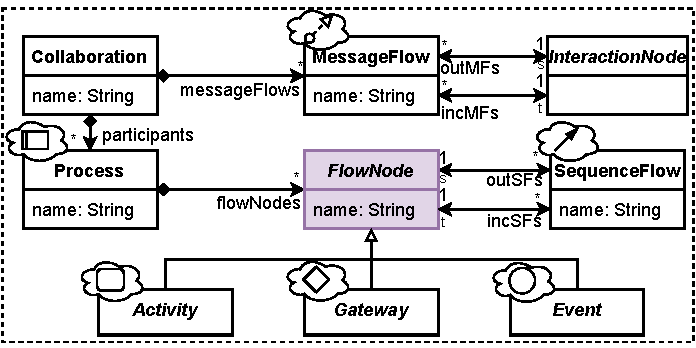
\includegraphics[width=0.9\linewidth]{images/bpmn_semantics-bpmn-metamodel.pdf}
  \caption{Excerpt of the \gls*{bpmn} metamodel \cite{objectmanagementgroupBusinessProcessModel2013}}
  \label{fig:bpmnMetamodel}
\end{figure}
% Containment: participants, messageFlows see fig. 9.33 in the BPMN spec.
% Containment: flowNodes (Process is FlowElementsContainer fig. 8.23). FlowElementsContainer have a containment of flowElements (also includes sequence flows)

A \gls*{bpmn} model is represented by a \textsf{Collaboration} that has \textsf{participants} and \textsf{messageFlows} between \textsf{InteractionNodes}.
Each participant is a \textsf{Process} containing \textsf{flowNodes} connected by \textsf{SequenceFlows}.
A \textsf{FlowNode} is either an \textsf{Activity}, \textsf{Gateway}, or \textsf{Event}.
Many types of \textsf{Activities}, \textsf{Gateways}, and \textsf{Events} exist.
Activities represent certain tasks to be carried out during a process, while events may happen during the execution of these tasks.
Furthermore, gateways model conditions, parallelizations, and synchronizations \cite{freundRealLifeBPMNUsing2019}.

The \gls*{bpmn} execution semantics is described using the concept of \textit{tokens} \cite{objectmanagementgroupBusinessProcessModel2013}, which can be located at sequence flows and specific flow nodes.
Tokens are consumed and created by flow nodes according to the connected sequence flows.
The \textsf{FlowNode} is colored purple in \autoref{fig:bpmnMetamodel} since it represents the \textit{state-changing elements} of \gls*{bpmn}, as described in \autoref{sec:formalization}.

A \gls*{bpmn} process is triggered by one of its start events, leading to a token at each outgoing flow of the triggered start event.
% Activities
Activities can start when at least one token is on an incoming sequence flow.
The start of an activity will move the incoming token to the activity.
When an activity terminates, it deletes its token and adds one at each outgoing sequence flow.
% Gateways
Furthermore, different gateway types exist, such as parallel and exclusive gateways.
Parallel gateways represent forks and joins, meaning they delete one token for each incoming sequence flow and add one token for each outgoing sequence flow.
Exclusive gateways represent an XOR by deleting a token from one incoming sequence flow and adding a token to exactly one of the outgoing sequence flows.
% Events (basic)
Events delete and add tokens similar to activities but have additional semantics depending on their type.
For example, message events will add or delete messages.

\subsection{Theoretical background}
We use typed attributed graphs for the formalization of the \gls*{bpmn} execution semantics.
Each state, \ie, token distribution during the execution of a \gls*{bpmn} model, is represented as an attributed graph typed by the \gls*{bpmn} execution type graph, which we introduce in \autoref{sec:formalization}.

Regarding \gls*{gt}, we utilize the single-pushout (SPO) approach with negative application conditions (NAC) \cite{ehrigALGEBRAICAPPROACHESGRAPH1997}, as implemented in Groove \cite{rensinkGROOVESimulatorTool2004}.
In addition, we utilize \textit{nested rules} with quantification to make parts of a rule repeatedly applicable or optional \cite{rensinkNestedQuantificationGraph2006,rensinkHowMuchAre2017}.
Moreover, we utilize the NACs to implement more intricate parts in the \gls*{bpmn} execution semantics, such as the termination of processes.

Formal definitions of SPO rules, their application, and the corresponding extensions of the theory (NACs, nested rules) are well-known, see \cite{ehrigALGEBRAICAPPROACHESGRAPH1997,rensinkNestedQuantificationGraph2006}.
We do not repeat them and instead focus on our practical contribution.


\section{BPMN semantics formalization} \label{sec:formalization}

The approach supports all the \gls*{bpmn} elements depicted in \autoref{fig:bpmnelementsOverview}.
These \gls*{bpmn} elements are divided into \textsf{Events}, \textsf{Gateways}, \textsf{Activities}, and \textsf{Edges}.
\textsf{Events} and \textsf{Activities} are further divided into subgroups.
Although all these elements have been implemented and tested (see \cite{krauterArtifactsLMCS2023}), we only explain the realization of the elements marked with a green or blue background due to space limitations.
The green elements were already described in \cite{krauterFormalizationAnalysisBPMN2023}, while explanations for the blue elements were added.
In the following, first, we define the \gls*{bpmn} execution metamodel to represent the \gls*{bpmn} state structure, then we explain our formalization of the elements in \autoref{fig:bpmnelementsOverview}.


\begin{figure}[ht]
    \centering
    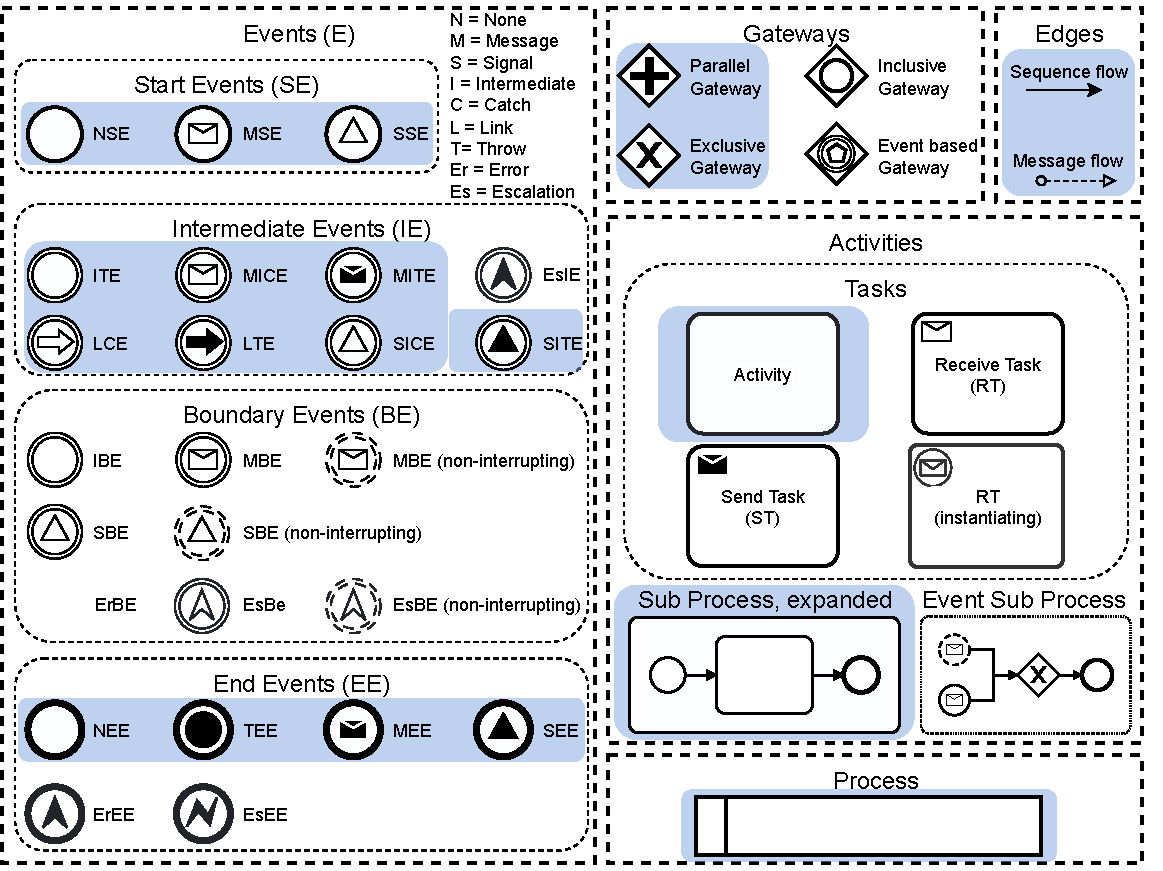
\includegraphics[width=0.99\textwidth]{images/bpmn_semantics-elements-overview.pdf}
    \caption{Overview of the supported \gls*{bpmn} elements (structure adapted from \cite{houhouFirstOrderLogicVerification2022})}
    \label{fig:bpmnelementsOverview}
\end{figure}


\subsection{BPMN execution metamodel}

In our formalization of BPMN, we utilize a token-based representation of the execution semantics, similar to the explanation in the informal description of the \gls*{bpmn} specification \cite{objectmanagementgroupBusinessProcessModel2013}.
To describe processes holding tokens during execution, we define the execution metamodel shown in \autoref{fig:typeGraph}, depicted as a UML class diagram.
In the context of our approach, we fulfill the role of the language engineer by defining the execution metamodel (see \autoref{fig:approach}).

\begin{figure}[ht]
  \centering
  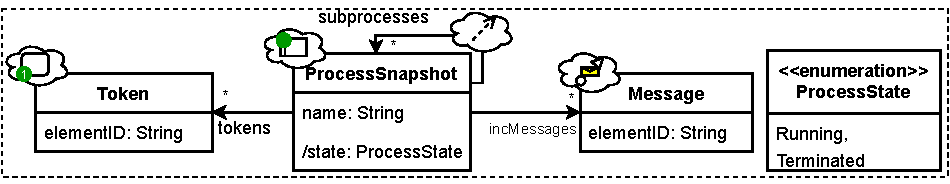
\includegraphics[width=1\linewidth]{images/bpmn_semantics-typegraph.pdf}
  \caption{BPMN execution metamodel}
  \label{fig:typeGraph}
\end{figure}

We use \textsf{ProcessSnapshot} to denote a running \gls*{bpmn} process with a specific token distribution that describes one state in the history of the process execution.
Every \textsf{ProcessSnapshot} has a set of \textsf{tokens}, incoming \textsf{messages}, and \textsf{subprocesses}.
A \textsf{ProcessSnapshot} has the state \textsf{Terminated} if it has no \textsf{tokens} or \textsf{subprocesses}.
Otherwise, it has the state \textsf{Running}.
A \textsf{Token} has an \textsf{elementID}, which points to the \gls*{bpmn} \textsf{Activity} or the \textsf{SequenceFlow} at which it is located.
A \textsf{Message} has an \textsf{elementID} pointing to a \textsf{MessageFlow}.
To concisely depict graphs conforming to this type graph, we introduce a concrete syntax in the clouds attached to the elements.
Our concrete syntax extends the \gls*{bpmn} syntax by adding process snapshots, subprocess relations, tokens, and messages.
Tokens are represented as colored circles drawn at their specified positions in a model.
In addition, we use colored circles at the top left of the bounding box, representing instances of the \gls*{bpmn} \textsf{Process}; these circles represent process snapshots.
The token's color must match the color of the process snapshot holding the token.
The concrete syntax was inspired by the bpmn-js-token-simulation \cite{camundaservicesgmbhBpmnjsTokenSimulation2023}.

Our BPMN execution metamodel was not created by extending the BPMN metamodel and adding missing concepts such as tokens and messages.
We chose to create a minimal execution model only containing concepts needed during execution.
This is only possible since our rules are generated by the \gls*{hot} for each specific BPMN model such that the structure of each model is already implicitly encoded in the rules.
This design choice leads to smaller states in the graph transformation system when compared to an execution metamodel that extends the BPMN metamodel.

The execution metamodel is a UML class diagram without operations, which can be seen as an attributed type graph \cite{heckelGraphTransformationSoftware2020}.
We keep the execution metamodel and the execution type graph separate (see \autoref{fig:approach}) because the execution metamodel should be independent of the formalism used to define the execution semantics.
One can reuse the execution metamodel when changing the formalism or concrete tool implementing the formalism (in our case, Groove) by adjusting how the execution metamodel is transformed.
Using the execution metamodel as the type graph, we can now define how the start graph and \gls*{gt} rules for the different \gls*{bpmn} elements are created.

Since our approach is based on a \gls*{hot} from \gls*{bpmn} to \gls*{gt} systems, we generate a \textit{start graph} and \textit{\gls*{gt} rules} for each given \gls*{bpmn} model (see \autoref{fig:approach}).
Generating the start graph for a \gls*{bpmn} model is straightforward.
First, for each process in the \gls*{bpmn} model, we generate a process snapshot if the process contains a \textit{none start event} (NSE).
An NSE describes a start event without a trigger (none).
Then, for each NSE, we add one token to each outgoing sequence flow.
An example of a start graph is shown in \autoref{fig:startGraph} using abstract and concrete syntax.

\begin{figure}[ht]
    \centering
    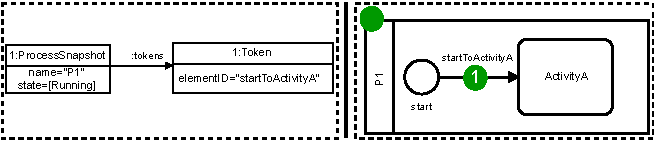
\includegraphics[width=0.85\textwidth]{images/startGraph.pdf}
    \caption{Example start graph in abstract (left) and concrete syntax (right)}
    \label{fig:startGraph}
\end{figure}

The \gls*{hot} generates one or more \gls*{gt} rules for each \textsf{FlowNode}, \ie, state-changing element in a \gls*{bpmn} model.
In order to provide a better understanding of the transformation process, we will begin by presenting example results, namely the generated rules for an activity.
Following this, we will delve into an explanation of how our \gls*{hot} creates these rules as well as rules for the other elements in \autoref{fig:bpmnelementsOverview}.

\autoref{fig:gtRuleAbstract} depicts an example \gls*{gt} rule ($L \to R$) to start an activity in abstract syntax.
The rule is straightforward, moving a token from the incoming sequence flow to the activity itself.

\begin{figure}[ht]
    \centering
  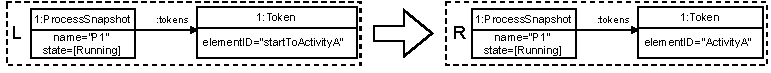
\includegraphics[width=1\textwidth]{images/rule_abstract.pdf}
  \caption{Example \gls*{gt} rule to start an activity (abstract syntax)}  \label{fig:gtRuleAbstract}
\end{figure}

For the rest of the article, we will depict all rules in the concrete syntax introduced earlier.
The rule from \autoref{fig:gtRuleAbstract} depicted in concrete syntax is shown on the left in \autoref{fig:gtRuleConcrete}.
The rule on the right in \autoref{fig:gtRuleConcrete} implements the termination of an activity, which will move one token from the activity to the outgoing sequence flow.

\begin{figure}[ht]
    \centering
  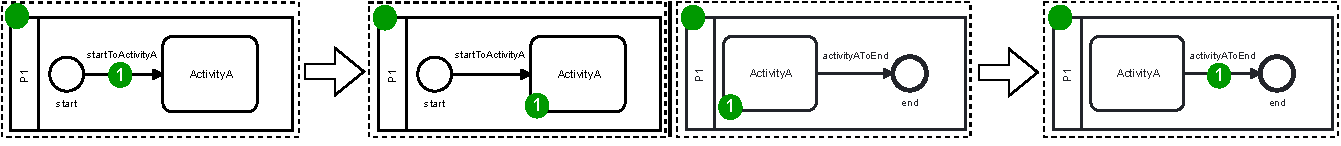
\includegraphics[width=1\textwidth]{images/rule_concrete.pdf}
  \caption{Example \gls*{gt} rule to start (left) and terminate (right) an activity}
  \label{fig:gtRuleConcrete}
\end{figure}

To summarize, we described two example rules and introduced a concrete syntax to depict them concisely and understandably.
In the following subsections, we use this concrete syntax to define how these rules and rules for other flow nodes are generated by our \gls*{hot}.
Elements of the \gls*{hot} are depicted using rule generation templates that show how specific rules are created for various flow nodes.
Defining the rule generation templates and thus the \gls*{hot} from \gls*{bpmn} to \gls*{gt} systems is the second task of the language engineer in our approach (see \autoref{fig:approach}).

Our \gls*{hot} defines a formal execution semantics of \gls*{bpmn}, similar to other approaches that formalize \gls*{bpmn} by mapping to Petri Nets or other formalisms \cite{dijkmanSemanticsAnalysisBusiness2008}.

\subsection{Process instantiation and termination} \label{subsec:instAndTermination}

Start events do not need \gls*{gt} rules since the generated start graph of the \gls*{gt} system will contain a token for each outgoing sequence flow of an NSE.
Other types of start events are triggered in corresponding throw event rules.

\autoref{fig:endTemplate} depicts the rule generation template for \textit{none end events} (\textsf{NEE}s in \autoref{fig:bpmnelementsOverview}).
All rule generation templates show a state-changing element (\textsf{FlowNode}) with surrounding flows in the left column and the applicable rule generation in the right column.
The left column shows instances of the \gls*{bpmn} metamodel (\autoref{fig:bpmnMetamodel}), and the right column shows the generated rules typed by the \gls*{bpmn} execution metamodel (see \autoref{fig:typeGraph}).
If more than one rule is generated from a \textsf{FlowNode}, an expression defines how each rule is generated.
For example, the expression $\forall \text{sf} \in \text{E.incSFs}$ for the rule generation template of end events (see \autoref{fig:endTemplate}) generates one rule for each incoming sequence flow \textit{sf} of the end event \textit{E}.
We use ``.'' in expressions to navigate along the associations of the \gls*{bpmn} metamodel shown in \autoref{fig:bpmnMetamodel}.
In the example, \textsf{E.incSFs} means following all \textsf{incSFs} links for a \textsf{FlowNode} object, resulting in a set of \textsf{SequenceFlow} objects.

\begin{figure}[ht]
    \centering
    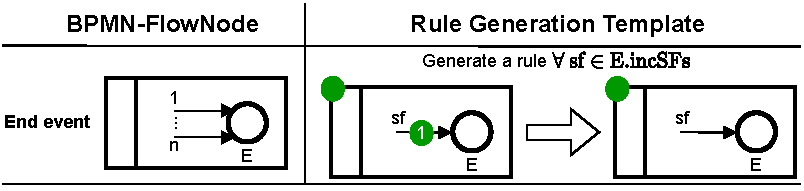
\includegraphics[width=1\textwidth]{images/end_template.pdf}
    \caption{Rule generation template for end events}
    \label{fig:endTemplate}
\end{figure}
    
% End Event
The generated end event rules delete tokens one by one for each incoming sequence flow.
However, they do not terminate processes.
% General termination rule
Process termination is implemented with a generic rule---independent of the input \gls*{bpmn} model---which is applicable to all process snapshots.
The termination rule in \autoref{fig:terminationRule} is automatically generated once during the \gls*{hot}.
The rule changes the state of the process snapshot from running to terminated if it has neither tokens nor subprocesses.

\begin{figure}[ht]
    \centering
    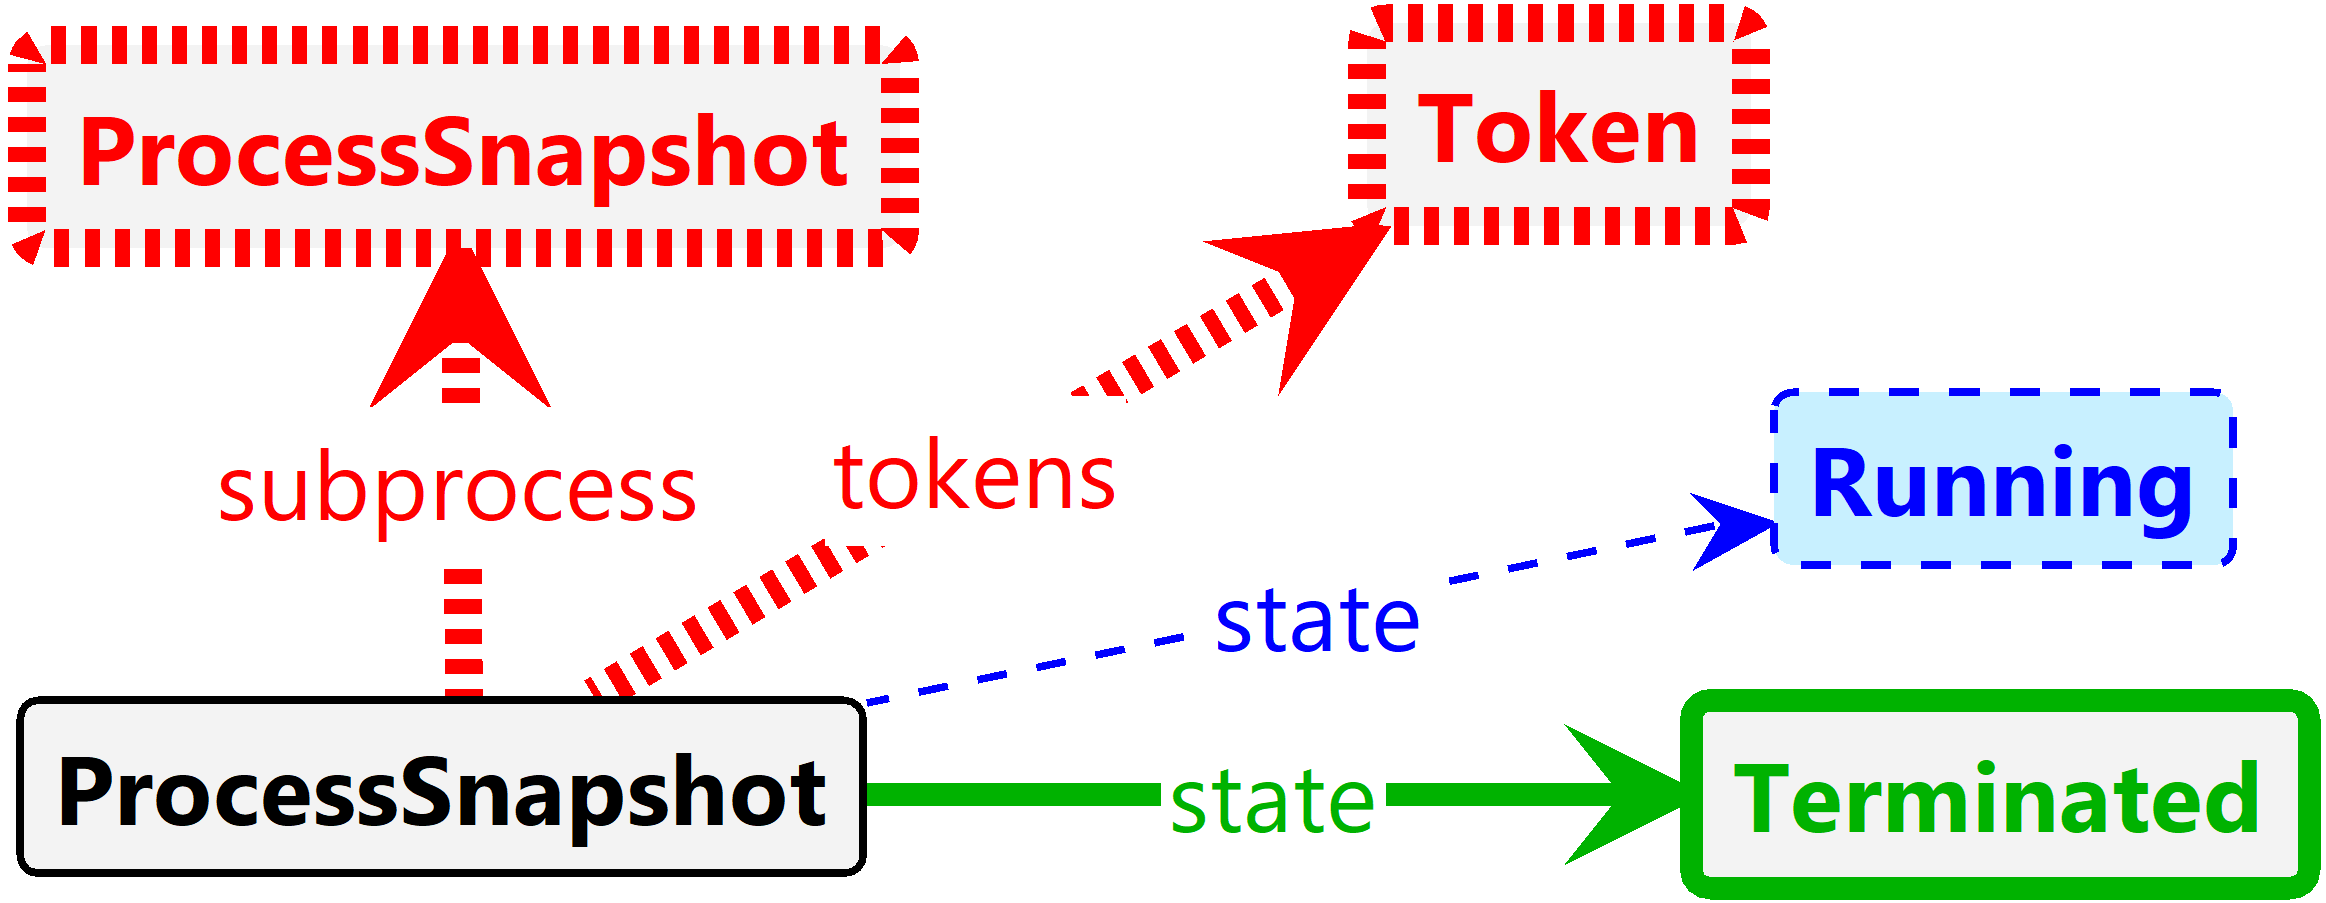
\includegraphics[width=.6\textwidth]{images/terminate_groove.png}
    \caption{Termination rule in Groove}
    \label{fig:terminationRule}
\end{figure}

The Groove syntax is the following.
The thin black elements in \autoref{fig:terminationRule} need to be present and will be preserved during transformation, while the dashed blue elements need to be present but will be removed.
Furthermore, the fat green elements will be created and the dashed fat red elements represent the NACs, whose presence prevent the rule from being applied.

\subsection{Activities \& Subprocesses}

% Normal activities
\autoref{fig:activityTemplates} depicts the rule generation templates for activities and subprocesses (see \autoref{fig:bpmnelementsOverview}).
Activity execution is divided into two steps implemented in two parts in the first rule template.
The upper part generates one rule for each incoming sequence flow to start the activity.
An activity can be started using a token positioned at any of its incoming sequence flows.
This part generates the sample rule on the right of \autoref{fig:gtRuleConcrete}.
Having multiple incoming or outgoing sequence flows for a flow node is considered bad practice since the implicitly encoded gateways should be explicit to avoid confusion.
Our formalization still supports those models not to force modelers to rewrite them, but we recommend using static analyzers to avoid such models \cite{camundaservicesgmbhBpmnlint2023}.

The lower part generates one rule that terminates the activity.
It deletes a token at the activity and adds one at each outgoing sequence flow.
This implicitly encodes a parallel gateway (see \autoref{fig:gatewayTemplates}) but should be avoided, as described earlier. 

% Could be split up into two figures
\begin{figure}[ht]
    \centering
    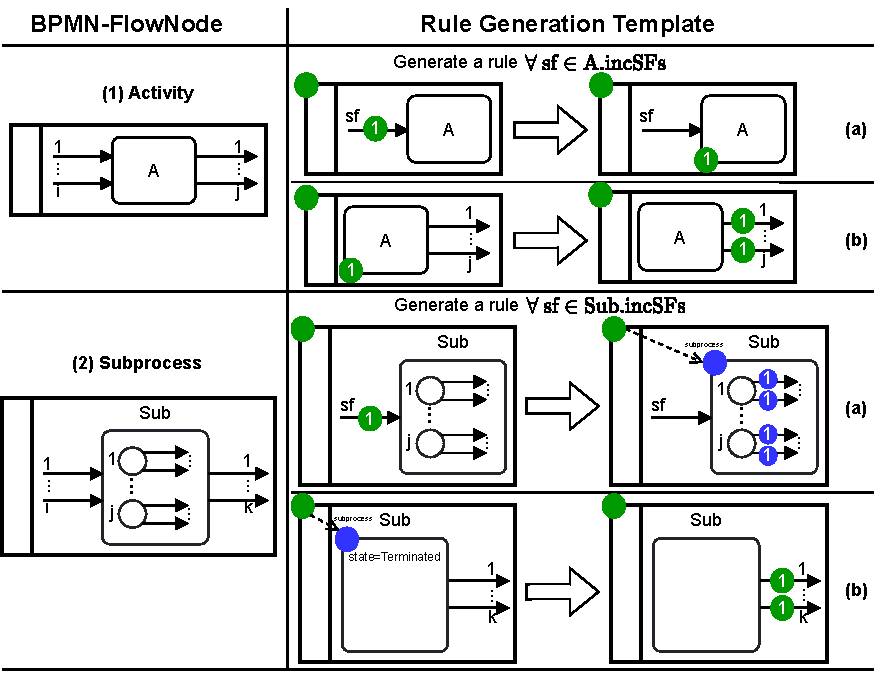
\includegraphics[width=1\textwidth]{images/activities_template.pdf}
    \caption{Rule generation template for activities and subprocesses}
    \label{fig:activityTemplates}
\end{figure}

% Subprocesses/Call activities
Subprocess execution is like activity execution.
The upper part of the template generates one rule for each incoming sequence flow.
The rule deletes an incoming token and adds a process snapshot representing a subprocess. 
The created process snapshot is represented with a colored circle on the top left corner of the subprocess with a token at each outgoing sequence flow of its start events (similar to start graph generation).
There is a \textit{subprocess} link between the process snapshots to depict the \textsf{subprocesses} relation in \autoref{fig:typeGraph}.
If the subprocess has no start events, a token will be added to every activity and gateway with no incoming sequence flows.

The bottom part of the template generates one rule to delete a terminated process snapshot and adds tokens at each outgoing sequence flow.
Subprocesses are terminated by the termination rule (see section \ref{subsec:instAndTermination}).


% Send/Receive tasks (mentioned/shown with message events later)
\subsection{Gateways}
\autoref{fig:gatewayTemplates} depicts the rule generation templates for parallel and exclusive gateways (see \autoref{fig:bpmnelementsOverview}).
A parallel gateway can synchronize and fork the control flow simultaneously.
Thus, one rule is generated that deletes one token from each incoming sequence flow and adds one token to each outgoing sequence flow.

\begin{figure}[ht]
    \centering
    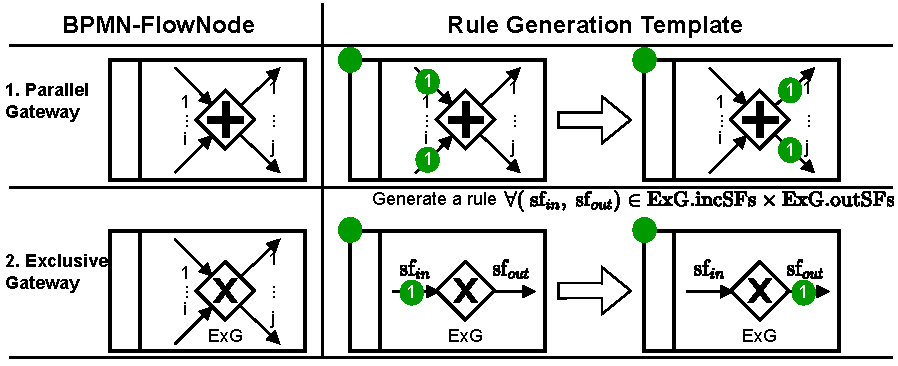
\includegraphics[width=1\textwidth]{images/gateways_template.pdf}
    \caption{Rule generation template for gateways}
    \label{fig:gatewayTemplates}
\end{figure}

Exclusive Gateways are triggered by exactly one incoming sequence flow, and exactly one outgoing sequence flow will be triggered as a result.
Thus, one rule must be generated for every combination of incoming and outgoing sequence flows.
However, the resulting rule is simple since it only deletes a token from an incoming sequence flow and adds one to an outgoing sequence flow.

\subsection{Message Events}
% General description
Message events are events directed at a single recipient.
Thus, they are unicast compared to broadcast signal events discussed later in \autoref{subsec:signalEvents}.
% Rule template description
% MITE
\autoref{fig:messageThrowEventTemplates} depicts the rule generation templates for \textit{message intermediate throw events} (\textsf{MITE} in \autoref{fig:bpmnelementsOverview}).
\textit{Message end events} (\textsf{MEE}) behave similarly to MITEs but only delete incoming tokens and do not add outgoing tokens.
% MITE with MICE
The first rule template describes how MITEs interact with \textit{message intermediate catch events} (MICEs).
A MITE deletes an incoming token and adds one at each outgoing sequence flow.
In addition, it sends one message to each process by adding it to the incoming messages of the process.
However, sending each message is optional, meaning that if a process is not ready to consume a message immediately, the message is not added.
A process can consume a message if its MICE has at least one token at an incoming sequence flow (see rule template two in \autoref{fig:messageThrowEventTemplates}).
We implement optional message sending using nested rules with quantification.
Concretely, we use an optional existential quantifier \cite{rensinkNestedQuantificationGraph2006} (see dotted rectangle labeled \textsf{Optional} in \autoref{fig:messageThrowEventTemplates}) to send a message only if the receiving process is ready to consume it.

% MITE with MSE
The second rule template describes how MITEs interact with MSEs.
For each MSE, a new process snapshot is created with tokens located at its outgoing sequence flows.
We split the interaction of MITEs with MICEs and MSEs into two rule templates for better understanding.
However, a MITE might interact with MICEs and MSEs simultaneously.
Thus, our \gls*{hot} implements a merge of both templates.

\begin{figure}[ht]
    \centering
    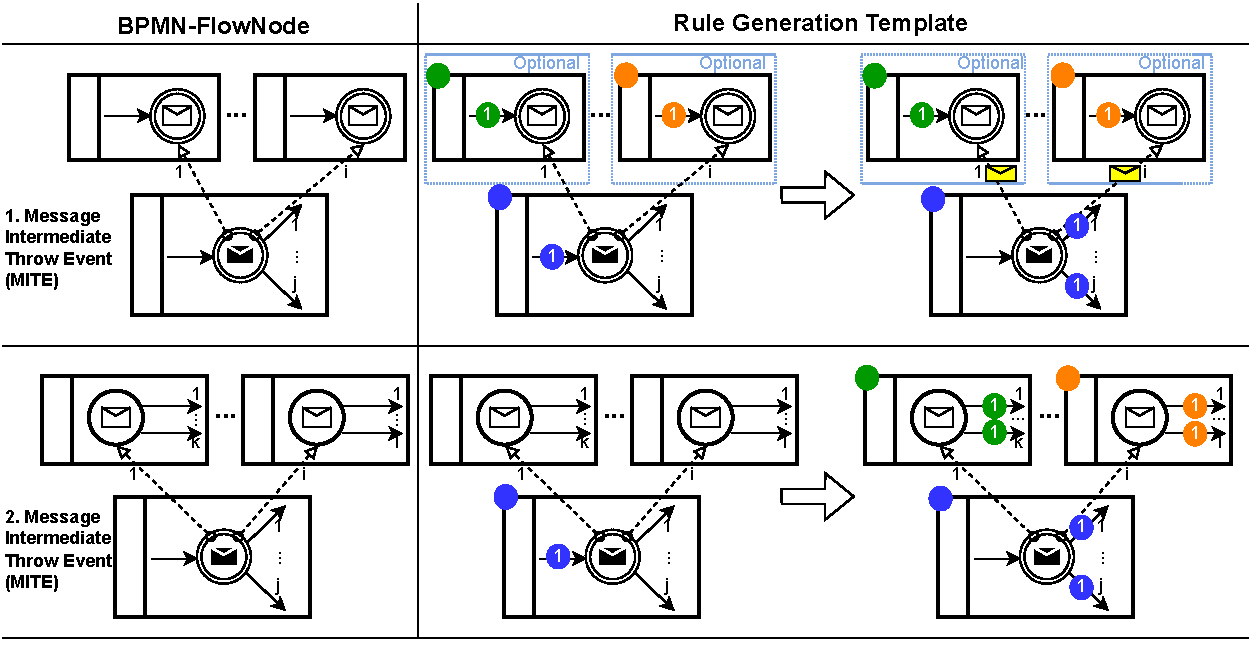
\includegraphics[width=1\textwidth]{images/mite_template.pdf}
    \caption{Rule generation templates for MITEs}
    \label{fig:messageThrowEventTemplates}
\end{figure}

% MICE
The template in \autoref{fig:messageCatchEventTemplates} shows the behavior of \textit{message intermediate catch events} (\textsf{MICE} in \autoref{fig:bpmnelementsOverview}).
To trigger a MICE, only one message at an incoming \textit{message flow} is needed.
Thus, one rule is generated for each incoming \textit{message flow}.
The rule template shows that MICEs delete one message and one token, as well as add a token at each outgoing sequence flow.

\begin{figure}[ht]
    \centering
    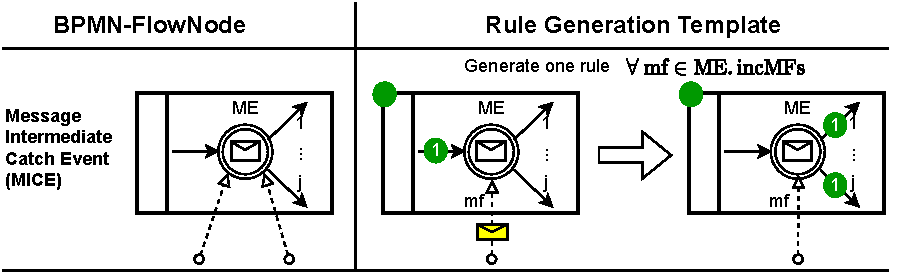
\includegraphics[width=0.8\textwidth]{images/mice_template.pdf}
    \caption{Rule generation templates for MICEs}
    \label{fig:messageCatchEventTemplates}
\end{figure}


\subsection{Link Events} \label{subsec:signalEvents}
% General description
Link events are similar to \enquote{Go To} statements since they move tokens from link throw events to link catch events in the same process level (cannot link to subprocesses).
They are meant to avoid long sequence flows and connect \gls{bpmn} models spanning multiple pages but can also be used to create loops due to their \enquote{Go To} nature \cite{objectmanagementgroupBusinessProcessModel2013}.
\autoref{fig:linkEventTemplates} depicts the rule generation templates for \textit{link throw events} and \textit{link catch events} (\textsf{LTE} and \textsf{LCE} in \autoref{fig:bpmnelementsOverview}).

\begin{figure}[ht]
    \centering
    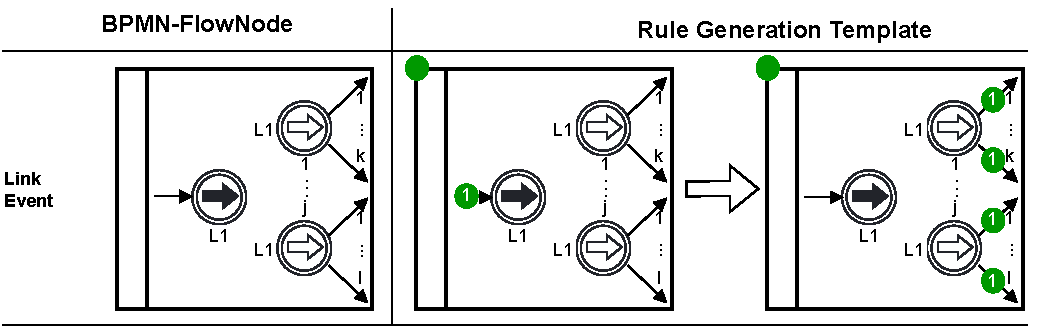
\includegraphics[width=1\textwidth]{images/linkEvent_template.pdf}
    \caption{Rule generation template for LTEs}
    \label{fig:linkEventTemplates}
\end{figure}

% Rule template description
Each rule deletes a token at that sequence flow and adds tokens to all outgoing sequence flows of matching LTEs.
An LTE matches an LCE if they have the same name.
In addition, they match despite different names if they have the same linked event definition (see \cite{objectmanagementgroupBusinessProcessModel2013}).
Our \gls*{hot} automatically finds matching LTEs during transformation and then applies the rule template shown in \autoref{fig:linkEventTemplates}.

\subsection{Signal Events}
% General description
Each signal event references a named signal.
Signal throw events \textit{broadcast} to all signal catch events with the same signal.
Signal broadcasts have a global scope, \ie, can communicate across process levels and pools \cite{objectmanagementgroupBusinessProcessModel2013}.

\autoref{fig:terminateEventTemplate} depicts the rule generation template for \textit{signal intermediate throw events} which interact with \textit{signal intermediate catch events} and \textit{signal start events} (\textsf{SITE}, \textsf{SICE}, and \textsf{SSE} in \autoref{fig:bpmnelementsOverview}).
\textit{Signal end events} (\textsf{SEE}) behave similarly to SITEs but only consume incoming tokens and do not add outgoing tokens.

\begin{figure}[ht]
    \centering
    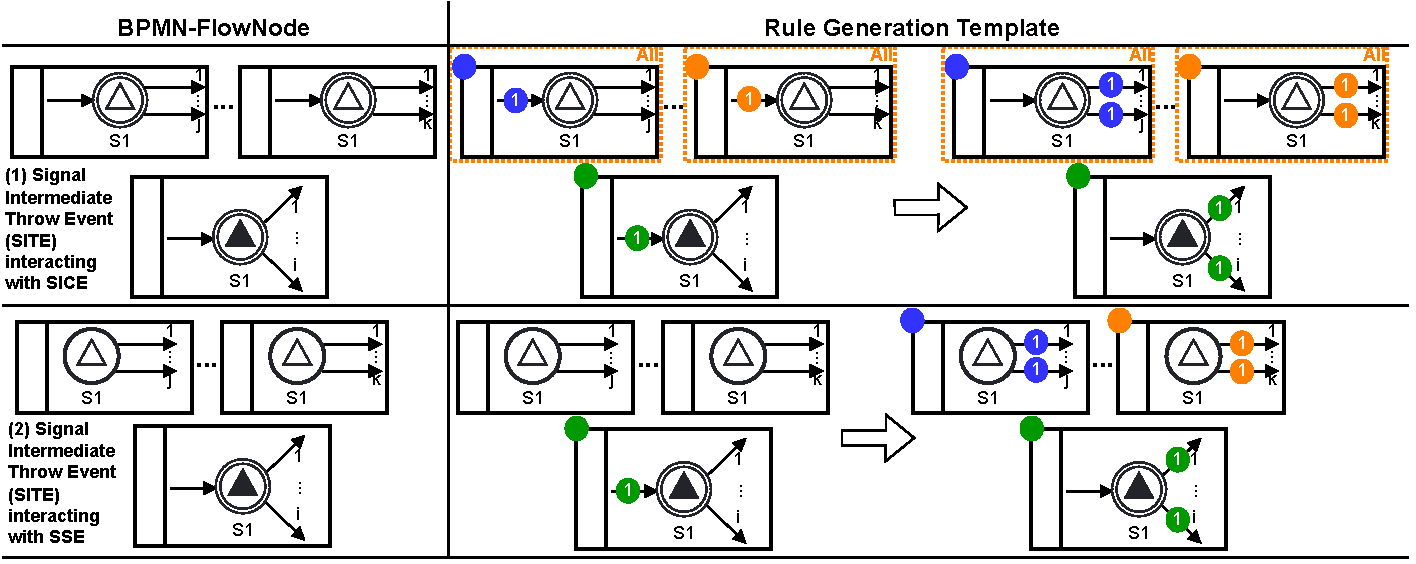
\includegraphics[width=1\textwidth]{images/signal_rule_template.pdf}
    \caption{Rule generation templates for SITEs}
    \label{fig:signalEventTemplates}
\end{figure}

% Rule template description
The first SITE template describes how SITEs interact with SICE.
Like other intermediate events, the incoming token is consumed while one token is added for each outgoing sequence flow.
Due to its broadcast semantics, a SITE interacts with all matching SICEs with an incoming token.
A SITE and SICE match if they have the same signal name.
In our templates, we assume that the signal name is the SITE/SICE name.
For each matching SICE, a universally quantified nested rule consumes the incoming token and adds a token for each outgoing sequence flow.
We use a universal quantifier since one process snapshot might have multiple tokens waiting before a SICE.
Then, a SITE should trigger this SICE multiple times.

The second SITE template describes how SITEs interact with SSEs.
Analogous to MITEs and MSEs a new process snapshots with tokens at the outgoing sequence flows of the SSEs is added for each matching SSE.
Each matching SSE is only triggered once, meaning we do not need any quantified nested rules.
% Merge of both templates
We split the interaction of SITEs with SICEs and SSEs into two rule templates for better understanding.
However, a SITE might interact with SICEs and SSEs simultaneously.
Thus, our \gls*{hot} implements a merge of both templates.

\subsection{Terminate Events}
% General description
A TEE abnormally terminates the running process \cite{objectmanagementgroupBusinessProcessModel2013}, meaning the process changes its state to terminated, and all its tokens are consumed.
\autoref{fig:terminateEventTemplate} depicts the rule generation template for \textit{terminate end events} (\textsf{TEE} in \autoref{fig:bpmnelementsOverview}).

\begin{figure}[ht]
    \centering
    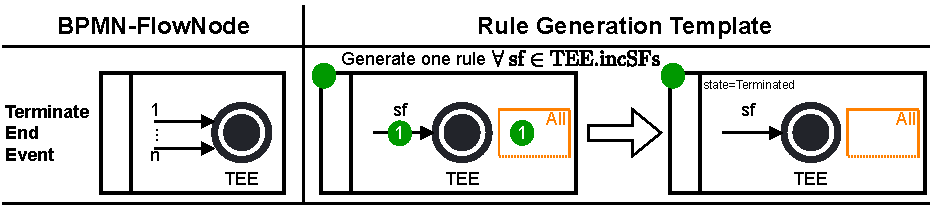
\includegraphics[width=0.8\textwidth]{images/terminate_end_event_template.pdf}
    \caption{Rule generation template for terminate end events}
    \label{fig:terminateEventTemplate}
\end{figure}

% Rule template description
One rule is generated for each incoming sequence flow of a TEE.
The rule consumes the incoming token, similar to the rules for end events, but also changes the process snapshot state to \textsf{Terminated}.
In addition, the rule deletes all other tokens of the process snapshot using a universally quantified nested rule (see dotted rectangle labeled \textbf{All} in \autoref{fig:terminateEventTemplate}).
Terminating a process must also terminate its subprocesses, which is not shown in the rule template but is described in our wiki \cite{krauterArtifactsLMCS2023}.

\section{Model checking BPMN} \label{sec:modelChecking}

Model checking---and verification in general---of \gls*{bpmn} models is necessary to ensure the correctness and reliability of business processes, which ultimately leads to increased efficiency, reduced costs, and user satisfaction.
Using our approach, model checking a \gls*{bpmn} model is possible using the generated \gls*{gt} system and behavioral properties based on atomic propositions (see \autoref{fig:approach}).
Behavioral properties are defined using a temporal logic, such as CTL and LTL.
In this article, we will use CTL.
An atomic proposition is formalized as a graph and holds in a given state if a match exists from the graph representing the proposition to the graph representing the state \cite{kastenbergModelCheckingDynamic2006}.

We differentiate between two types of behavioral properties: \textit{general \gls*{bpmn} properties} defined for all \gls*{bpmn} models and \textit{custom properties} tailored towards a particular \gls*{bpmn} model.
We do not consider structural properties (like conformance to the syntax of BPMN) since they can be checked using a standard modeling tool without implementing execution semantics.
We will now give an example of two predefined general \gls*{bpmn} properties and show how they can be checked using our approach.
Then, we describe how custom properties can be defined and checked.

\subsection{General BPMN properties}
\textit{Safeness} and \textit{Soundness} properties are defined for \gls*{bpmn} in \cite{corradiniClassificationBPMNCollaborations2018}.
A \gls*{bpmn} model is \textit{safe} if, during its execution, at most one token occurs along the same sequence flow \cite{corradiniClassificationBPMNCollaborations2018}.
Soundness is further decomposed into (i) \textit{Option to complete}: any running process instance must eventually complete, (ii) \textit{Proper completion}: after completion, each token of the process instance must be consumed by a different end event, as well as (iii) \textit{No dead activities}: each activity can be executed in at least one process instance \cite{corradiniClassificationBPMNCollaborations2018}.
Process completion is synonymous with process termination.
In the following, we will describe how to implement the \textit{Safeness} and \textit{Option to complete} properties.

% Safeness
We specify \textit{Safeness} as the CTL property defined in \eqref{eq:safeness}.
The atomic proposition \textsf{Unsafe} is true if two tokens of one process snapshot point to the same sequence flow.
It is shown in \autoref{fig:unsafe} using abstract Groove syntax.
We cannot use the concrete syntax to define the \textsf{Unsafe} proposition because the proposition should apply to any BPMN model.
Our concrete syntax is always used with a given BPMN model.

\begin{figure}[ht]
    \centering
    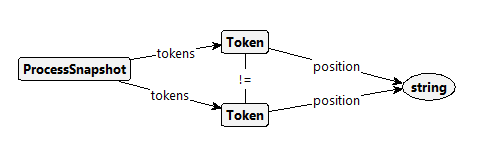
\includegraphics[width=0.8\textwidth]{images/Unsafe.png}
    \caption{The atomic proposition \textit{Unsafe} in Groove.}
    \label{fig:unsafe}
\end{figure}

\begin{figure}[ht]
    \centering
    
\includegraphics[width=0.5\textwidth]{images/AllTerminated.png}
    \caption{The atomic proposition \textit{AllTerminated} in Groove.}
    \label{fig:allTerminated}
\end{figure}

% Option to complete
\textit{Option to complete} is specified using the CTL property defined in \eqref{eq:optionToComplete}.
The atomic proposition \textsf{AllTerminated} is true if there exists no process snapshot in the state \textsf{Running}, \ie, all process snapshots are \textsf{Terminated}.
It is shown in \autoref{fig:allTerminated} using abstract Groove syntax.

\noindent\begin{minipage}{.5\linewidth}
\begin{equation} \label{eq:safeness}
  AG(\neg \,\text{Unsafe})
\end{equation}
\end{minipage}%
\begin{minipage}{.5\linewidth}
\begin{equation} \label{eq:optionToComplete}
  AF(\text{AllTerminated}) 
\end{equation}
\end{minipage}
\vskip.3\baselineskip

Checking the properties \textit{Safeness}, \textit{Option to Complete}, and \textit{No Dead Activities} is implemented in our tool \cite{krauterArtifactsLMCS2023}.
The property \textit{Proper Completion} is not yet implemented, but all the information needed can be found in the \gls*{gt} systems state space.

\subsection{Custom properties} \label{subsec:customProperties}
% Defining atomic propositions in BPMN is a novelty.
To make model checking user-friendly, we envision modelers defining atomic propositions based on the extended \gls*{bpmn} syntax, \ie, the concrete syntax introduced in \autoref{fig:typeGraph}.
Therefore, to define an atomic proposition, a modeler adds process snapshots and tokens to a \gls*{bpmn} model, which we can automatically convert to a \gls*{gt} rule representing an atomic proposition.
\gls*{gt} rules representing atomic propositions are not allowed to delete or add elements and are called graph conditions in Groove.
Furthermore, a modeler can define that a token should not exist at a given position, which leads to NAC's in the graph condition. 

For example, the token distribution shown in \autoref{fig:shippedTwiceProposition} defines a process snapshot with two tokens at activity \textit{Ship goods}.
A modeler could use this atomic proposition to check if the activity \textit{Ship goods} is executed twice by creating an appropriate LTL/CTL property.
Shipping goods twice but only receiving one payment during an order-handling process would be a critical error for a business.
The order handling process in \autoref{fig:shippedTwiceProposition} is taken from \cite{ruckerPracticalProcessAutomation2021} but changed to contain a modeling error.
The modeling error leads to potentially shipping goods twice if the process is not corrected before deployment.

\begin{figure}[ht]
    \centering
    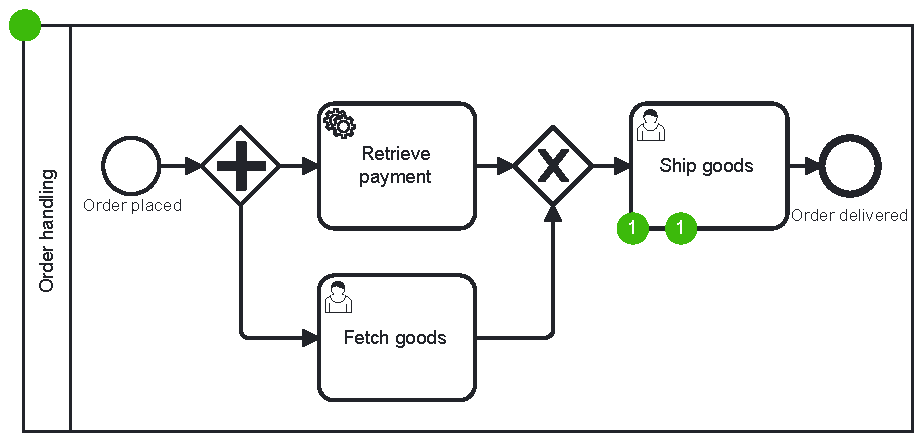
\includegraphics[width=0.65\textwidth]{images/shippedTwiceProposition.pdf}
    \caption{Atomic proposition defining shipping goods twice.}
    \label{fig:shippedTwiceProposition}
\end{figure}

Another proposition for the same erroneous process is shown in \autoref{fig:shippingAfterPayment}.
The proposition defines that when the activity \textit{Ship goods} runs (has a token) the activity \textit{Retrieve payment} should not run (has no token).
\enquote{Has no token} is depicted by crossing out the token symbol and represents an extension of our concrete syntax introduced for defining propositions.
This proposition can be used to define a property to check if shipping ever occurs while retrieving payments has not been completed yet.
The \gls*{gt} system for the order handling process containing both propositions can be found in \cite{krauterArtifactsLMCS2023}.

\begin{figure}[ht]
    \centering
    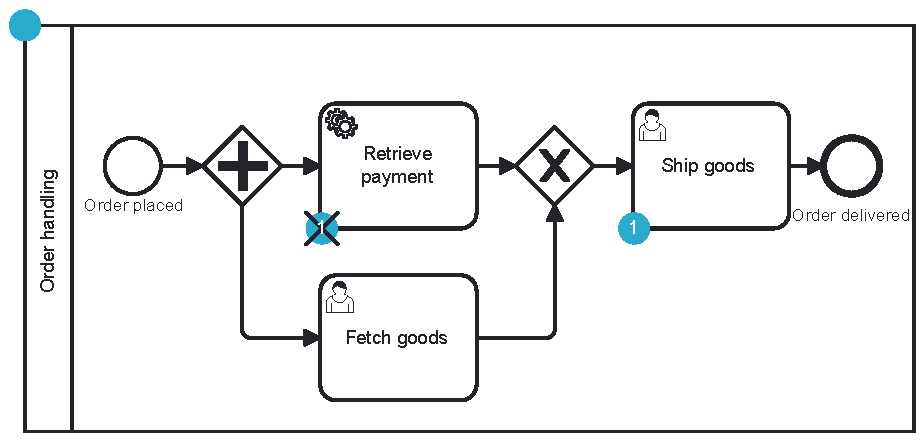
\includegraphics[width=0.65\textwidth]{images/shippingAfterPayment.pdf}
    \caption{Atomic proposition defining shipping after retrieving payment.}
    \label{fig:shippingAfterPayment}
\end{figure}

Using a proposition editor based on our concrete syntax, a modeler can work with \gls*{bpmn}, which is well-known to him.
He does not need to define his propositions in the \gls*{gt} semantics used for execution since each proposition is automatically transformed as described earlier.
To summarize, many propositions can defined using this simple method.
However, the expressibility is not the same as in the \gls*{gt} semantics.
For example, one can use nested rules with quantification in graph conditions in Groove.
Thus, when defining a proposition editor, there is a clear tradeoff between \textit{simplicity} and \textit{expressibility}.
Currently, we favor simplicity in our tool and recommend defining propositions in \gls*{gt} semantics if more powerful constructs are needed.
In addition, expressibility varies and is achieved differently in \gls*{gt} tools, and we try to stay as independent as possible from specific \gls*{gt} tools.

Finally, the modeler must still know the temporal logic, such as LTL and CTL, to express his properties.
To combat this problem, we added temporal logic templates to our tool to generate commonly occurring propositions without knowledge about temporal logic.
This feature is discussed in detail in the implementation section.
In the future, a domain-specific property language for \gls*{bpmn} would further lessen the knowledge required from the modeler \cite{meyersProMoBoxFrameworkGenerating2014}.

\section{Implementation} \label{sec:impl}
In this section, we will present our tool and the improvements we made since \cite{krauterFormalizationAnalysisBPMN2023}.
In addition, we describe experiments regarding its performance.

\subsection{BPMN Analyzer tool}

Our approach is implemented in a web-based tool called \textit{\gls*{bpmn} Analyzer}, which is open-source, publicly available, and does not require any installation \cite{krauterArtifactsLMCS2023, krauterFormalizationAnalysisBPMN2023}.
\autoref{fig:implScreenshot} depicts a screenshot of the \gls*{bpmn} Analyzer.
We use the order handling process from \cite{ruckerPracticalProcessAutomation2021} as an example.
It is the same \gls*{bpmn} model as in \autoref{fig:shippedTwiceProposition} and \autoref{fig:shippingAfterPayment} but without modeling errors.

The modeler can create or upload a \gls*{bpmn} model, which can then be verified using either general \gls*{bpmn} properties or custom CTL properties.
BPMN Analyzer can generate a \gls*{gt} system for the supplied \gls*{bpmn} model and run model checking in Groove \cite{kastenbergModelCheckingDynamic2006}. 
To evaluate the correctness of our \gls*{hot}, we have created a comprehensive test suite \cite{krauterArtifactsLMCS2023}.
It verifies that rules are generated as defined by the rule generation templates in the previous section for each \gls*{bpmn} element.

\begin{figure}[ht]
    \centering
    \frame{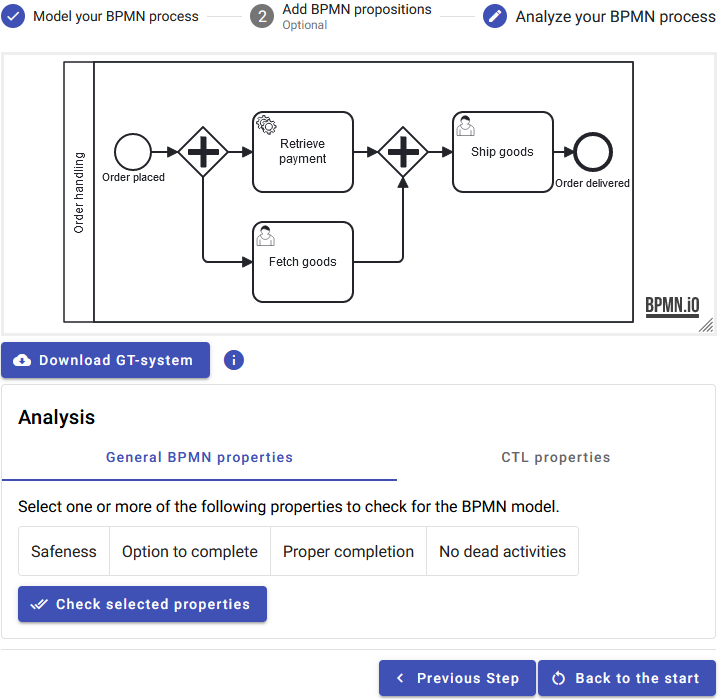
\includegraphics[width=1\textwidth]{images/impl_step3.png}}
    % 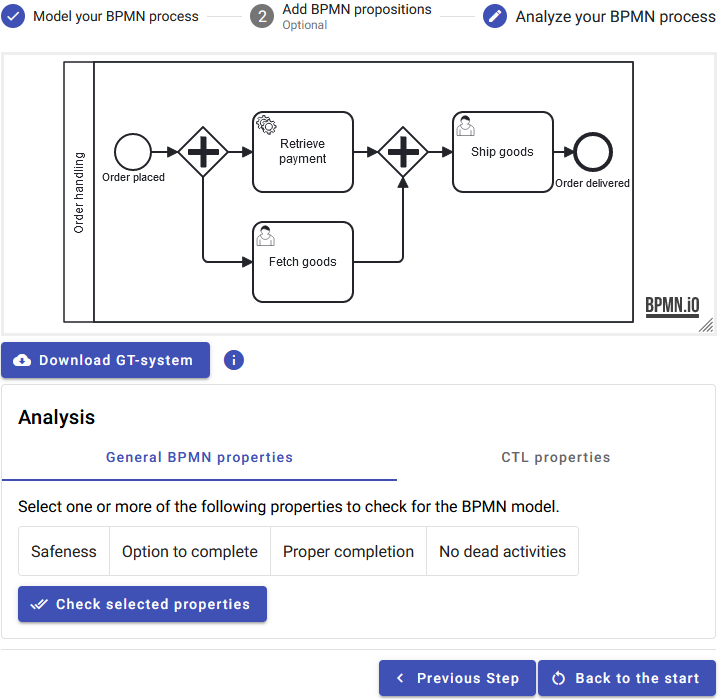
\includegraphics[width=1\textwidth]{images/impl_step3.png}
    \caption{Screenshot of the \textit{analysis step} in the BPMN Analyzer tool}
    \label{fig:implScreenshot}
\end{figure}

We significantly improved the \gls*{bpmn} Analyzer tool for this extended version.
First, we improved the usability of the tool.
We restructured the user interface, previously contained on one page, into three distinct steps while adding new features.
The user is transparently guided through these three steps by the application flow.

(1) The \textbf{Modeling} step lets a user upload or define his \gls{bpmn} model.
We integrated a properties panel into the modeling step such that a user does not need another tool to view and edit the IDs of \gls*{bpmn} elements.
This allows for better traceability between \gls*{bpmn} elements and generated \gls*{gt} rules when a user chooses to inspect the \gls*{gt} system.

(2) The \textbf{Custom Propositions} steps contains the new proposition editor.
In this step, a user can create as many propositions as needed for custom temporal logic properties.
If a user is only interested in general \gls*{bpmn} properties, he can skip this step.
Each proposition is created using the introduced visual concrete syntax.
To create a proposition, a user attaches tokens and process snapshots to the \gls*{bpmn} model created in the modeling step.
We implemented a custom diagram editor for this step to achieve the best possible usability.

(3) In the final \textbf{Analysis} step the user can check the mentioned general \gls*{bpmn} properties and write CTL properties.
The propositions defined in the second step are listed and available for the CTL model checking.
If a user chooses to download the generated \gls*{gt} system, it will also contain the defined propositions converted to graph conditions.

Second, we added CTL templates to the analysis of the step such that a modeler can generate commonly occurring CTL propositions.
He selects a template and a proposition to generate a CTL property.
So far, we have added two templates for checking if a state (described by a proposition) can be reached or is never reached.
Thus, simple safety and liveness properties can be checked using these templates.
Model-checking experts in an organization can define more templates in the future and share them for reuse. 

Third, we published multiple parts of our application as libraries such that they can be reused seamlessly by other researchers and practitioners \cite{krauterArtifactsLMCS2023}.
The \gls*{bpmn} execution metamodel needed for the definition of custom propositions is published as an npm module (\textit{token-bpmn-moddle}).
In addition, the token-based proposition editor is also published as an npm module (\textit{token-bpmn}).
Furthermore, we published our \gls*{gt} rule generation library to the maven central repository (\textit{graph-rule-generation}).
The library currently contains an implementation to generate \gls*{gt} rule for Groove but could also be used for other graph transformation tools in the future.

\subsection{Experiments}

Model checking is a useful technique but often falls short in practice due to insufficient performance.
Poor performance might have many reasons, most notably large models leading to state space explosion.
We experimented with ten different \gls*{bpmn} models from \cite{houhouFirstOrderLogicVerification2022} to assess the performance of our implementation.
We picked the models at random, besides disregarding some similar models.
The models include realistic business process models (001, 002, and 020) \cite{houhouFirstOrderLogicVerification2022}.

To calculate the average runtime, we used the hyperfine benchmarking tool \cite{peterHyperfine2022} (version 1.18.0), which ran the \gls*{hot}/state space exploration for each \gls*{bpmn} model ten times.
The experiment was run on Windows 11 (AMD Ryzen 7700X processor, 32 GB RAM) using Groove version 6.1.0 \cite{krauterArtifactsLMCS2023}.
Compared to \cite{krauterFormalizationAnalysisBPMN2023}, we used the newest \gls*{hot} implementation and the newest Groove and hyperfine versions.

First, we ran our \gls*{hot} for the \gls*{bpmn} models.
The \gls*{hot} takes approximately half a second to generate a \gls*{gt} system for each model.
Thus, the generation of the \gls*{gt} systems for these models is fast enough.

Second, we ran a full state exploration using the resulting ten \gls*{gt} systems, see \autoref{table:stateSpaceBenchmark}.
The exploration takes around one second for most of the models.
Only model \textit{020} needs nearly two seconds due to its larger state space.
Furthermore, up to one second is spent on startup, not model checking.
For example, Groove reports only 722 ms for state space exploration for model \textit{020}.

We conclude that our approach is sufficiently fast for models of average size.
In addition, there is still room for optimization, such as avoiding costly I/O to disk or parallelizing the \gls*{hot}.
In the next section, we test the scalability of our approach.
However, a comprehensive benchmark, including a detailed comparison to other tools, is left for future work.

\begin{table}[ht]
\centering
\caption[Experimental results for a full state space exploration in Groove]{Experimental results for a full state space exploration in Groove}

\begin{tabular}{| c | c | c || c | c | c |}
 \hline
 BPMN model & Processes & Nodes (gw.) & States & Transitions & Total time \\
 \hline\hline
 001 & 2 & 17(2) & 68 & 118 & $\sim$ 1.00 s \\
 \hline
 002 & 2 & 16(2) & 62 & 108 & $\sim$ 0.97 s \\
 \hline
 007 & 1 & 8(2) & 45 & 81 & $\sim$ 0.92 s \\
 \hline
 008 & 1 & 11(2) & 49 & 85 & $\sim$ 0.93 s \\
 \hline
 009 & 1 & 12(2) & 137 & 308 & $\sim$ 1.01 s \\
 \hline
 010 & 1 & 15(2) & 162 & 357 & $\sim$ 1.04 s \\
 \hline
 011 & 1 & 15(2) & 44 & 69 & $\sim$ 0.97 s \\
 \hline
 015 & 1 & 14(2) & 53 & 86 & $\sim$ 0.95 s \\
 \hline
 016 & 1 & 14(2) & 44 & 68 & $\sim$ 0.94 s \\
 \hline
 020 & 1 & 39(6) & 3060 & 8584 & $\sim$ 1.75 s \\
 \hline
\end{tabular}
\label{table:stateSpaceBenchmark}
\end{table}

\section{Scalability test} \label{sec:scalability}

In this section, we test the scalability of our approach by applying it to 300 \gls*{bpmn} models with increasing model size. 

\subsection{Setup}

We generated 300 \gls*{bpmn} to test the scalability of our approach.
We used the following approach to include different \gls*{bpmn} elements in our models.
We generated the models incrementally, increasing the number of \textit{blocks} they contain.
Thus, model one contains one block, model two contains two blocks, and so forth until the last model contains 300 blocks.
During the generation, we alternate between the three different blocks shown in \autoref{fig:blocks}.

\begin{figure}[ht]
    \centering
    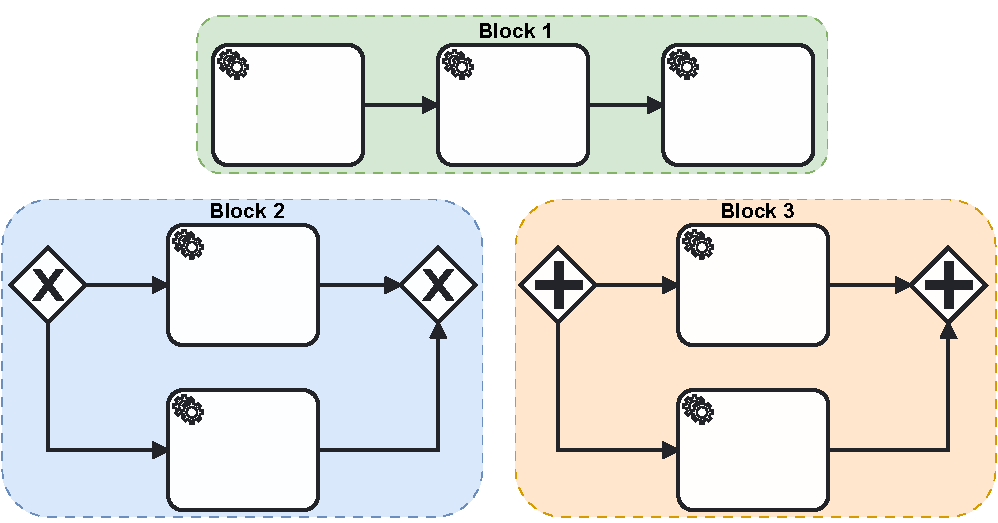
\includegraphics[width=0.9\textwidth]{images/blocks.pdf}
    \caption{Different blocks for BPMN model generation}
    \label{fig:blocks}
\end{figure}

For example, the \gls*{bpmn} model with three blocks is depicted in \autoref{fig:threeBlockModel}.
We then repeat adding one block at a time for each new model until we reach 300 models.

\begin{figure}[ht]
    \centering
    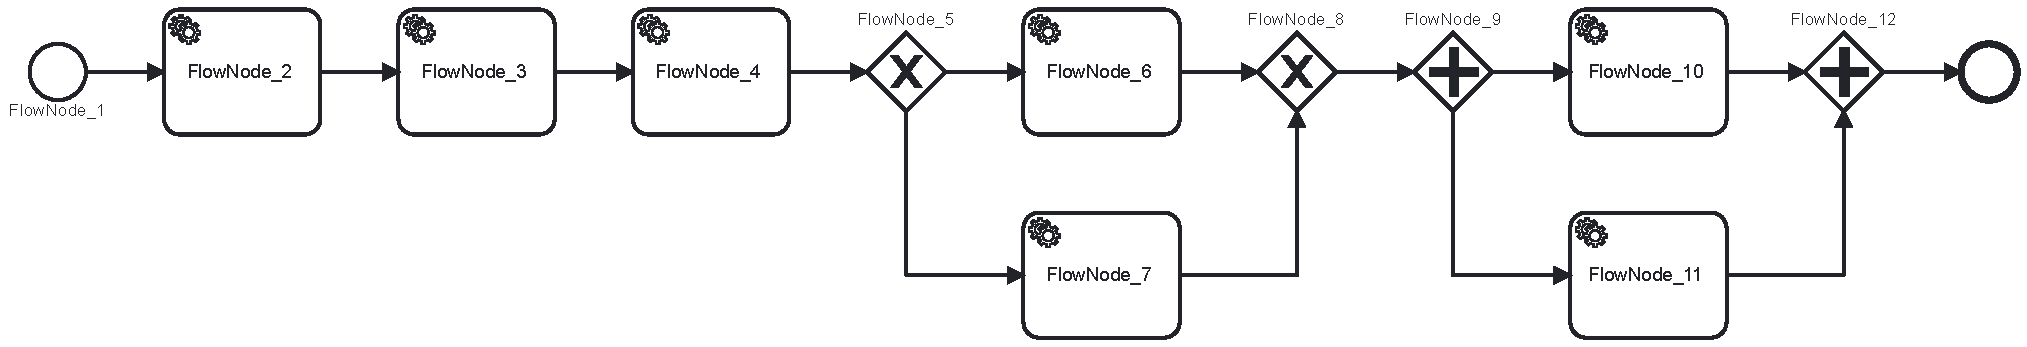
\includegraphics[width=1\textwidth]{images/003.pdf}
    \caption{A generated BPMN model with three blocks}
    \label{fig:threeBlockModel}
\end{figure}

\autoref{table:inputModels} states the characteristics of the generated BPMN models, such as the number of gateways, flow nodes, and sequence flows.
One can deduce from the table that adding fifty blocks adds around 400 \gls*{bpmn} elements to a model.
All models, including their characteristics and how to generate them, can be found in \cite{krauterArtifactsLMCS2023}.

The \gls*{bpmn} modeling tools we have used are already struggling with models that have 200 or more blocks.
Thus, we stopped at 300 blocks since we think \gls*{bpmn} models in practice are much smaller and so we could still run our benchmark in reasonable time.
\gls*{bpmn} models are developed together by the business and development people of an organization.
Consequently, large models are divided into smaller submodels such that they are still understandable by humans.
From our experience this best practice leads to tiny models compared to our scalability test. 

\begin{table}[ht]
\centering
\caption[Generated BPMN model characteristics]{Generated BPMN model characteristics}
\begin{tabular}{| c | c | c | c || c |}
 \hline
 BPMN model / Blocks & Gateways & Flow nodes & Sequence flows & Total elements \\
 \hline\hline
 1 & 0 & 5 & 4 & 9 \\
 \hline
 50 & 66 & 185 & 217 & 402 \\
 \hline
 100 & 132 & 368 & 433 & 801 \\
 \hline
 150 & 200 & 552 & 651 & 1203 \\
 \hline
 200 & 266 & 735 & 867 & 1602 \\
 \hline
 250 & 332 & 918 & 1083 & 2001 \\
 \hline
 300 & 400 & 1102 & 1301 & 2403 \\
 \hline
\end{tabular}
\label{table:inputModels}
\end{table}

\subsection{Results}

% Description
\autoref{fig:hotScalability} depicts the results of benchmarking our \gls*{hot} with the generated \gls*{bpmn} models.
It shows the average runtime of five runs for transforming each \gls*{bpmn} model, calculated by hyperfine \cite{peterHyperfine2022}.
We used the same machine and setup as discussed for our performance experiments in \autoref{sec:impl}.

\begin{figure}[ht]
    \centering
    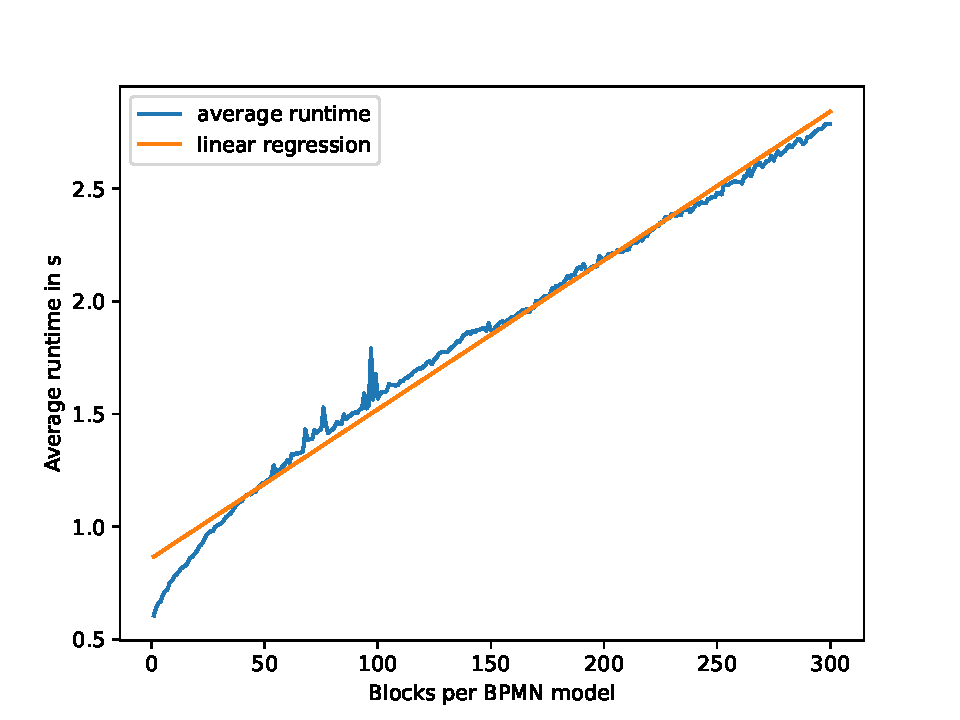
\includegraphics[width=0.7\textwidth]{images/HOT_scalability.pdf}
    \caption{HOT scalability results}
    \label{fig:hotScalability}
\end{figure}

% Interpretation and take aways
% Looks linear as expected O(n) where n is the number of flow nodes(for loop for each flow-node).

% Description
\autoref{fig:stateSpaceScalability} depicts the results of benchmarking the state space generation in Groove for the \gls*{gt}-systems obtained by our \gls*{hot}.
It shows the average runtime of five runs, calculated by hyperfine \cite{peterHyperfine2022}.

\begin{figure}[ht]
    \centering
    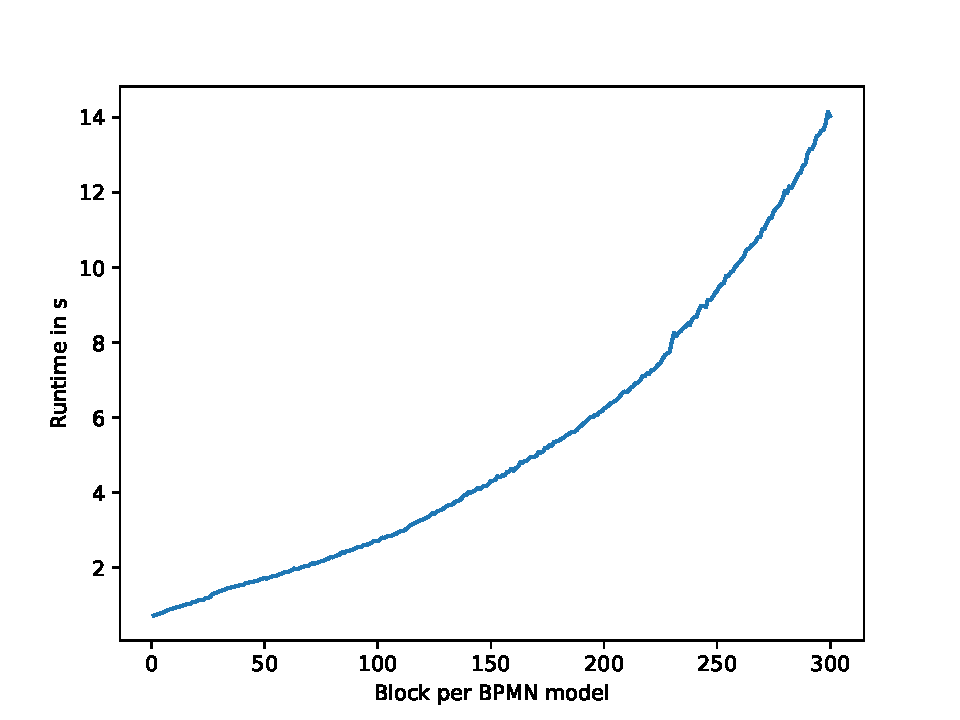
\includegraphics[width=0.7\textwidth]{images/StateSpaceGeneration_scalability.pdf}
    \caption{State space scalability results}
    \label{fig:stateSpaceScalability}
\end{figure}

% Interpretation and take aways

\section{Related work} \label{sec:relatedWork}
% Petri nets formalisms
The most common formalizations of \gls*{bpmn} use Petri Nets.
For example, \cite{dijkmanSemanticsAnalysisBusiness2008} formalize a subset of \gls*{bpmn} elements by defining a mapping to Petri Nets conceptually close to our \gls*{hot}-based formalization.
% Difficulties with Petri net encodings
Encoding basic \gls*{bpmn} modeling elements into Petri Nets is generally straightforward, but for some advanced elements, it can be complicated to define \cite{hofstedeWorkflowPatternsExpressive2002}.
For example, representing \textit{termination end events} and \textit{interrupting boundary events}, which interrupt a running process, is usually unsupported because of the complexity of managing the non-local propagation of tokens in Petri Nets \cite{corradiniFormalApproachAnalysis2021}.
We solve these situations by using nested graph conditions, for example, to remove all tokens when reaching a \textit{termination end event}.

% Van gorp
A \gls*{bpmn} formalization based on in-place \gls*{gt} rules is given in \cite{vangorpVisualTokenbasedFormalization2013}.
The formalization covers a substantial part of the \gls*{bpmn} specification, including complex concepts such as inclusive gateways and compensation.
In addition, the \gls*{gt} rules are visual and thus can be aligned with the informal description of the execution semantics of BPMN.
A key difference to our approach is that the rules in \cite{vangorpVisualTokenbasedFormalization2013} are general and can be applied to every \gls*{bpmn} model, while we generate specific rules for each \gls*{bpmn} model using our \gls*{hot}.
Thus, our approach can be seen as a program specialization compared to \cite{vangorpVisualTokenbasedFormalization2013} since we process a concrete \gls*{bpmn} model before its execution.
However, they do \textit{not} support property checking since their goal is only formalization.

% BProve/Corradini
The tool \textit{BProVe} is based on formal \gls*{bpmn} semantics given in rewriting logic and implemented in the Maude system \cite{corradiniFormalApproachAnalysis2021}.
Using this formal semantics, they can verify custom LTL properties and general \gls*{bpmn} properties, such as Safeness and Soundness.

% fbpmn/Houhou
The verification framework \textsf{fbpmn} uses first-order logic to formalize and check \gls*{bpmn} models \cite{houhouFirstOrderLogicVerification2022}.
This formalization is then realized in the TLA\textsuperscript{+} formal language and can be model-checked using TLC.
Like BProVe, \textsf{fbpmn} allows checking general \gls*{bpmn} properties, such as Safeness and Soundness.
Furthermore, they focus on different communication models besides the standard in the \gls*{bpmn} specification and support time-related constructs.
We currently disregard time-related constructs \cite{duranVerifyingTimedBPMN2017,houhouFirstOrderLogicVerification2022} and data flow \cite{corradiniFormalisingAnimatingMultiple2022,el-saberCMMICMComplianceChecking2015}.

\autoref{tab:supportedelements} shows which \gls*{bpmn} elements are supported by our approach and the approaches mentioned above.
Compared to other approaches, we cover most \gls*{bpmn} elements.
The coverage of \gls*{bpmn} elements greatly impacts how useful each approach is to check properties in practice.
In addition, we cover the most important elements found in practice since we come close to the element coverage of popular process engines such as Camunda \cite{camundaservicesgmbhBPMNImplementationReference2023}.

The missing elements, when compared to Camunda, are transactions, cancel events, and compensation events.
These elements are rather complex, but \cite{vangorpVisualTokenbasedFormalization2013} shows how cancel and compensation events can be formalized.
We plan to support these elements by extending our implementation and test suite in the future.

\begin{table}[htbp]
    \caption{\gls*{bpmn} elements supported by different formalizations (based on \cite{vangorpVisualTokenbasedFormalization2013}).}
    \label{tab:supportedelements}
    \begin{threeparttable}
    \begin{tabular}{l l l l l l}
    \hline
      \gls*{bpmn} element/feature & Dijkman & Van Gorp &  Corradini & Houhou & This\\
      & \cite{dijkmanSemanticsAnalysisBusiness2008} & \cite{vangorpVisualTokenbasedFormalization2013} & \cite{corradiniFormalApproachAnalysis2021}&  \cite{houhouFirstOrderLogicVerification2022} & article\\
      \hline
      \textit{Instantiation and termination}\\
      Start event instantiation & X & X & X & X & X\\
      Exclusive event-based gateway & & X & & & X \\
        \quad instantiation \\
      Parallel event-based gateway & & & & & \\
        \quad instantiation \\
      Receive task instantiation & & & & & X\\
      Normal process completion & X & X & X & X & X\\
      \\
      \textit{Activities}\\
      Activity & X & X & X & X & X\\
      Loop activity & X & X & & &\\
      Multiple instance activity & & & & & \\
      Subprocess & X & X & & X & X\\
      Event subprocess & &  &  &  & X\\
      Transaction & &  &  &  & \\
      Ad-hoc subprocesses & & & & &\\
      \\
      \textit{Gateways}\\
      Parallel gateway & X & X & X & X & X\\
      Exclusive gateway & X & X & X & X & X\\
      Inclusive gateway (split) & X & X & X & X & X\\
      Inclusive gateway (merge) & & X & & X & X\\
      Event-based gateway & & & X\tnote{1} & X & X\\ % No timer and conditional events after event based gateway supported.
      Complex gateway & & & & &\\
      \\
      \textit{Events} \\
      None Events & X & X & X & X & X\\
      Message events & X & X & X & X & X\\
      Timer Events & & & & X & \\
      Escalation Events & & & & & X\\
      Error Events & X & X & & & X\\
      Cancel Events & & X & & &\\
      Compensation Events & & X & & &\\
      Conditional Events & & & & &\\
      Link Events & & X & & & X\\
      Signal Events & & X & & & X\\
      Multiple Events & &  & & & \\
      Terminate Events & & X & X & X & X\\
      Boundary Events & & X\tnote{2} & & X\tnote{3} & X\\ % To the same extent as the event support
    \end{tabular}
    \begin{tablenotes}
        \item[1] Does not support receive tasks after event-based gateways.
        \item[2] Only supports interrupting boundary events on tasks, not subprocesses.
        \item[3] Only supports message and timer events.
    \end{tablenotes}
    \end{threeparttable}
\end{table}


\section{Conclusion \& future work} \label{sec:conclusion}
This article makes two main practical contributions.
First, we conceptualize a new approach utilizing a \gls*{hot} to formalize the semantics of behavioral languages.
Our approach moves complexity from the \gls*{gt} rules to the rule templates making up the \gls*{hot}.
Furthermore, the approach can be applied to any behavioral language if one can define its \textit{state structure} and identify its \textit{state-changing elements}.

Second, we apply our approach to BPMN, resulting in a comprehensive formalization regarding element coverage (compared to the literature and industrial process engines) that supports checking behavioral properties.
Furthermore, our contribution is implemented in an open-source web-based tool to make our ideas easily accessible to other researchers and practitioners.

Future work targets both of our main contributions.
First, we plan a detailed comparison of our \gls*{hot} approach with approaches that utilize fixed rules.
It will be interesting to investigate how the two approaches differ, for example, in runtime during state space generation.
Second, we aim to improve our formalization and the resulting tool in multiple ways.
We intend to extend our formalization to support the remaining few \gls*{bpmn} elements used in practice and want to turn the modeling environment of our tool into an interactive simulation environment.
In addition, we can use this environment to visualize potential counterexamples in cases where behavioral properties are violated.

% TODO: Add after review
% \section*{Acknowledgment}
%   \noindent We want to thank the anonymous reviewers for their valuable comments and helpful suggestions.
  
\bibliographystyle{alphaurl} 
\bibliography{bib}

\end{document}
